%!TEX root=../oi-magistr-spolecne.tex
\section[PAL - Vyhledávání v textu, automaty]{Přesné a přibližné hledání množin vzorků v textu, Hammingova a Levenshteinova vzdálenost. Efektivní algoritmy hledání založené na využití konečných automatů. Klasické hledání v textu (naivní, Boyer-Moore). Slovníkové automaty.}

\begin{itemize}
\item \textbf{Abeceda:} Konečná množina znaků. Značí se $A$
\item \textbf{Text:} Posloupnost znaků nad danou abecedou. Symboly textu se značí $t_1, \hdots, t_n$
\item \textbf{Vzorek:} Posloupnost znaků nad stejnou abecedou, jejich výskyt se hledá v daném textu. Text bývá řádově delší než vzorek. Symboly vzorku se značí $p_1, \hdots, p_m$
\end{itemize}

\subsection{Hammingova vzdálenost}
Hammingova vzdálenost $k \geq 0$, je minimální číslo takové, že změnou symbolů na $k$ různých pozicích v jednom z řetězců získáme druhý řetězec. Symboly nelze vypouštět nebo přidávat, Hammingova vzdálenost je \textbf{definována} jen pro \textbf{řetězce stejné délky}. V praxi se implementuje pomocí dynamického programování podobně jako Levenshteinova vzdálenost. Využití při vyhledávání podřetězců.

\begin{figure}[h]
    \begin{center}
        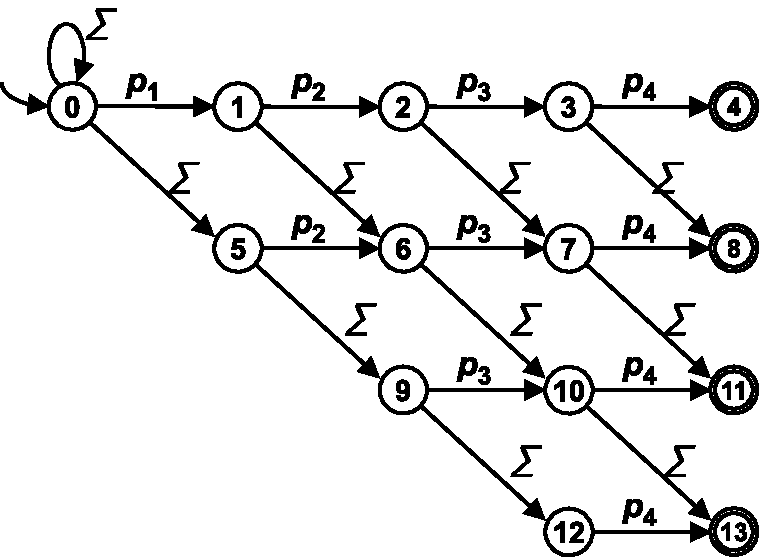
\includegraphics[width=60mm]{spolecne/04/images/hamming-automat}
    \end{center}
    \caption{NFA, který přijímá slovo s Hammingovou vzdáleností max 3 od vzoru $p_1p_2p_3p_4$}
\end{figure}

\subsection{Levenshteinova vzdálenost}
Levenshteinova vzdálenost je minimální počet operací \textbf{vkládání, mazání a substituce} takových, aby po jejich provedení byly zadané řetězce totožné. Používá se dynamické programování (předpočítaná tabulka).

\paragraph{Vyplnění tabulky:}

\begin{enumerate}
\item v nultém řádku a sloupcy tabulky $A$ jsou postupně inkrementované čísla od 0
\item pokud jsou znaky na pozici $(i,j)$ shodné, vložíme na pozici $(i,j)$ hodnotu $A(i-1, j-1)$
\item pokud se znaky liší, na pozici $(i,j)$ vložíme minimum z těchto tří hodnot:
\begin{enumerate}
\item $A(i,j-1)+1$ - odpovídá operaci odstranění znaku
\item $A(i-1,j)+1$ - odpovídá operaci vložení znaku
\item $A(i-1,j-1)+1$ - odpovídá operaci substituce znaku
\end{enumerate}
\item Výsledky najdeme v posledním řádku tabulky. Zajímají nás sloupce, kde je hodnota menší rovna požadované Levenshteinově vzdálenosti. Čteme zprava doleva.
\end{enumerate}


\begin{table}[h]
\begin{tabular}{|l|l|l|l|l|l|l|l|l|l|}
\hline
           &   & \textbf{S} & \textbf{a} & \textbf{t} & \textbf{u} & \textbf{r} & \textbf{d} & \textbf{a} & \textbf{y} \\ \hline
           & 0 & 1          & 2          & 3          & 4          & 5          & 6          & 7          & 8          \\ \hline
\textbf{S} & 1 & \textbf{0} & \textbf{1} & \textbf{2} & 3          & 4          & 5          & 6          & 7          \\ \hline
\textbf{u} & 2 & 1          & 1          & 2          & \textbf{2} & 3          & 4          & 5          & 6          \\ \hline
\textbf{n} & 3 & 2          & 2          & 2          & 3          & \textbf{3} & 4          & 5          & 6          \\ \hline
\textbf{d} & 4 & 3          & 3          & 3          & 3          & 4          & \textbf{3} & 4          & 5          \\ \hline
\textbf{a} & 5 & 4          & 3          & 4          & 4          & 4          & 4          & \textbf{3} & 4          \\ \hline
\textbf{y} & 6 & 5          & 4          & 4          & 5          & 5          & 5          & 4          & \textbf{3} \\ \hline
\end{tabular}
\vspace{15px}
\caption{Levenshteinova vzdálenost slova \uv{Sunday} a \uv{Saturday} = 3}
\end{table}

\subsection{Hledání v textu pomocí konečných automatů}

\paragraph{Deterministický konečný automat (DFA)} je automat, který z každého stavu může přejít do maximálně jednoho cílového stavu.

\paragraph{Nedeterministický konečný automat (NFA)} je automat, který z každého stavu může přejít do libovolného počtu cílových stavů. Po přečtení jednoho symbolu ze vstupu přejde současně do všech cílových stavů a ze všech těchto stavů pokračuje čtením dalšího vstupu. V přechodové tabulce NKA je navíc sloupeček pro prázdný vstup, označovaný $\epsilon$ (prázdné slovo; $\epsilon~\sum$). Epsilon-přechody automat provádí neustále bez čtení symbolu ze vstupu.

DFA i NFA jsou definovány jako pětice ${A, Q, q_0, F, \delta}$, kde $A$ je vstupní konečná abeceda, $Q$ je množina vnitřních stavů, $q_0$ je počáteční, $F$ je neprázdná množina koncových stavů, $\delta$ je přechodová funkce.

\paragraph{Přechodová funkce:}
\begin{itemize}
\item V DFA je $\delta : Q \times A \rightarrow Q$
\item V NFA je $\delta : Q \times A \rightarrow P(Q)$, kde $P$ je potenční množina
\end{itemize}

\begin{figure}[h]
    \begin{center}
        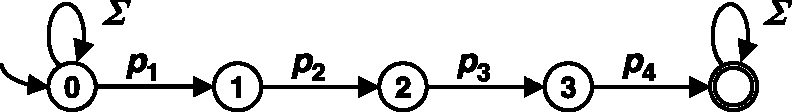
\includegraphics[width=100mm]{spolecne/04/images/automat-hledani}
    \end{center}
    \caption{NFA, který přijímá jakékoliv slovo se substringem $p_1p_2p_3p_4$ (kdekoliv)}
\end{figure}

\paragraph{Převod NFA do DFA} Opisuju všechny stavy + přidávám nově vzniklé \uv{multistavy}. Tabulka může narůst až na $2^n$ stavů.

\paragraph{Operace s automaty:} S tím souvisí $\epsilon$-přechod. To je takový přechod, který se děje neustále, bez přečtení vstupu.
\begin{itemize}
\item \textbf{union} - vytvoří se nový start stav a do obou start stavů sjednocovaných automatů se vytvoří $\epsilon$-přechod
\item \textbf{concatenation} - z finálních stavů A se vytvoří $\epsilon$-přechody do start stavů B
\item \textbf{iteration} - nový start stav s $\epsilon$-přechodem do startu A; z finálních stavů A $\epsilon$-přechody do startů A.
\item \textbf{intersection} - kartézský součin stavů z obou automatů
\end{itemize}

\subsection{Naivní hledání}
\begin{enumerate}
\item Přiložíme vzorek k začátku textu.
\item Dokud znaky vzorku a textu souhlasí, posunujeme se ve vzorku kupředu.
\item Když narazíme na neshodu, posuneme celý vzorek o jednu pozici kupředu, ve vzorku se nastavíme na začátek a jdeme na 2.
\item Když dojdeme za konec vzorku nebo vzorek přesáhne za konec textu, ohlásíme výsledek a případně postupujeme dále jako ve 3.
\end{enumerate}

Složitost tohoto postupu je $O(m \cdot n)$, kde $m$ je délka vzoru a $n$ je délka textu.

\subsection{Boyer-Moore}
\begin{enumerate}
\item Vzorek přiložíme k textu a testujeme shodu vzorku odzadu.
\item Když dojde k neshodě, je šance, že vzorek lze posunout o více pozic dopředu, mnohdy o celou délku vzorku. Čím delší vzorek, tím rychlejší hledání!
\end{enumerate}
\paragraph{Kolize na poslední pozici vzorku}
Dopomáhá nám tabulka BCS (bad character shift). BCS je tabulka indexovaná znaky abecedy značící vzdálenost znaků od konce vzorku. Když tam znak není, je vzdálenost délka vzorku.

\begin{figure}[h]
    \begin{center}
        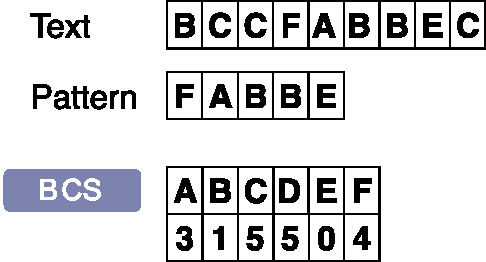
\includegraphics[width=50mm]{spolecne/04/images/bcs}
    \end{center}
\end{figure}

\paragraph{Kolize po částečné shodě na konci vzorku} Nastávají 3 případy:

\begin{itemize}
\item Přípona $p$ se ve vzorku vyskytuje, a to tak, že jí předchází jiný znak než právě ve vzorku kolidující. Pak musíme vzorek posunout tak, aby se tato další nejbližší instance přípony kryla s textem, tj. o vzdálenost mezi těmito instancemi přípony.
\item Některá přípona vzorku stejně dlouhá nebo kratší než $p$ se vyskytuje také na začátku vzorku. Uvažme nejdelší takovou příponu, označme její výskyt na začátku vzorku symbolem $q$. Vzorek pak musíme posunout o vzdálenost mezi $p$ a $q$.
\end{itemize}

Tabulka GSS (Good Suffix Shift) obsahuje přípony vzorku všech možných délek od 1 do $m$, kde $m$ je délka vzorku a k těmto příponám počet pozic, o které se má vzorek posunout v případě kolize.

\begin{figure}[h]
    \begin{center}
        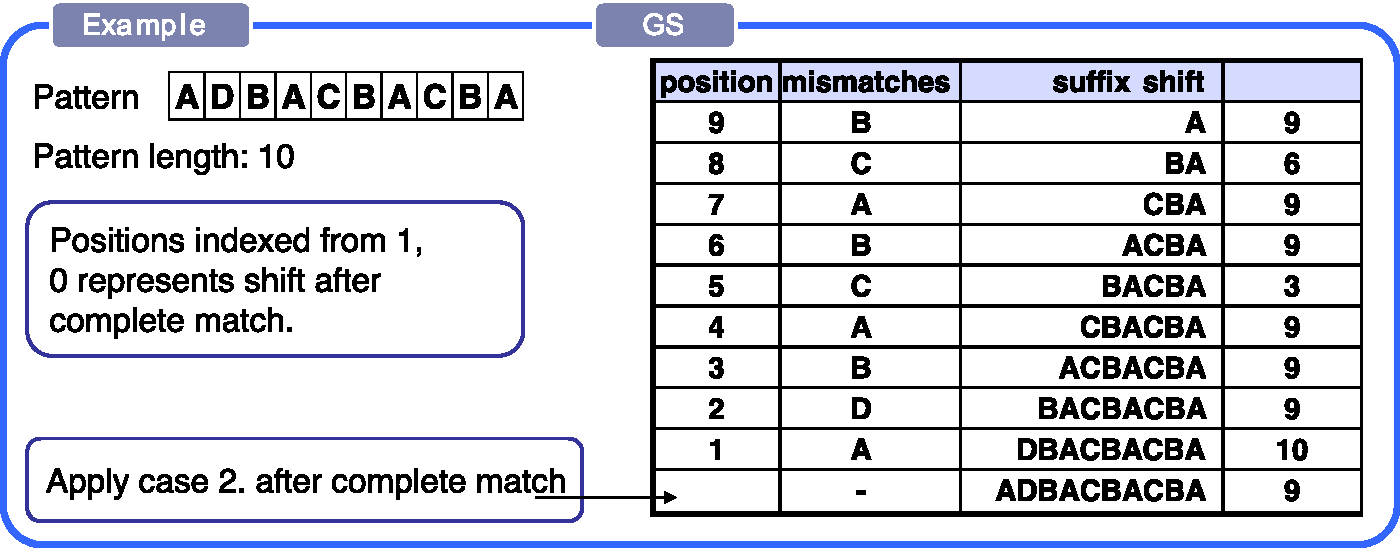
\includegraphics[width=120mm]{spolecne/04/images/gss}
    \end{center}
\end{figure}


\subsection{Slovníkové automaty}
Slovník nad abecedou A je konečná množina řetězců (patternů) z A*. Slovníkový automat hledá text pro jakýkoliv řetězec ve slovníku.

\begin{itemize}
\item Abeceda: A = \{a, c, d, e, g, h, i, l, m, n, o, q, r, s, t, u, v, y\}
\item Slovník: D = \{add, advanced, algorithms, to, your, algonqiuan, adventures\}
\end{itemize}

Stejné prefixy se dají mergovat do společných stavů.

\begin{figure}[h]
    \begin{center}
        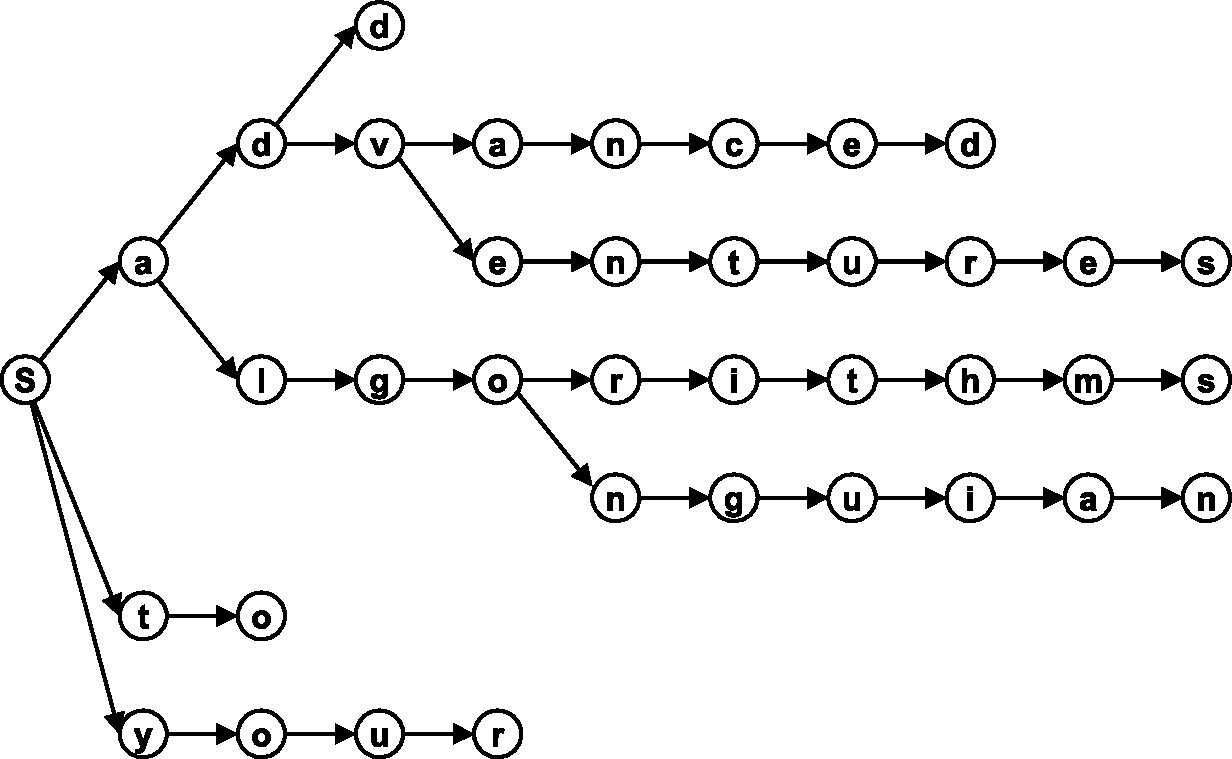
\includegraphics[width=120mm]{spolecne/04/images/slovnikovy-automat}
    \end{center}
    \caption{Slovníkový automat (bez suffix vylepšení)}
\end{figure}

\paragraph{Vylepšení:} Identické suffixy lze mergovat do jednoho stavu, např. \uv{add} - lze zrušit jeden stav (koncové \uv{d}) a dát přechod do jiného koncového \uv{d} (např. u slova \uv{advanced}).